% Latex template for submission to the 16th International Meeting on Fully 3D Image Reconstruction 
% in Radiology and Nuclear Medicine (Fully3D 2021)
%
% re-used for 2025 meeting, thanks Georg!
%
% Author: G.Schramm
% Date:   Oct 2020
%
% 
% To build this document, we recommend to use latexmk via:
% ```latexmk -pdf fully3d_template.tex```
% Building in the online editor overleaf also works.

\documentclass[11pt,twocolumn,twoside]{article}
\usepackage{fully3d}

%%%%%% add your extra packages here (if needed)                                       %%%%%
%%%%%% before, have a look which packages are already imported by the fully3d package %%%%%
%\usepackage{mypackage}


%%%%% add your bibtex file that contains the bibtex entries here %%%%%
%%%%% please include DOIs in the bibtex entries if possible      %%%%%
\addbibresource{fully3d_template.bib}

\begin{document}


%-------------------------------------------------------------------------------------------
%%%%% add your title here %%%%%
\title{LaTex Template for Fully3D 2025 submission} 

%%%%% add authors and affiliations here %%%%%
\author[1]{First~Author}
\author[1,2]{Second~Author}
\author[2]{Third~Author}

\affil[1]{Department of Nuclear Medicine,
          University of Reconstruction, City, Country}

\affil[2]{Department of Radiology,
          Recon University, City, Country}

%%%%% don't change these 2 lines %%%%%
\maketitle
\thispagestyle{fancy}



%-------------------------------------------------------------------------------------------
%%%%% add your summary (abstract) here               %%%%%%
%%%%% use footnotesize for this section              %%%%%%
%%%%% please stick to the customabstract environment %%%%%% 


\begin{customabstract}
Please insert your abstract here. This abstract can be slightly longer than the very short 150-word version required for the online submission system. 

\bigskip

\textbf{\textit{\color{red}Include a sentence about the novelty and impact to medical imaging.}}

\end{customabstract}


%-------------------------------------------------------------------------------------------
%%%%% main text                                                %%%%%    
%%%%% remove the dummy content and put your own content here   %%%%% 
%%%%% feel free to choose your own section titles              %%%%% 
%%%%% you don't need to put the content in a separate tex file %%%%%

% dummy_content.tex shows how to add sections, figures, tables, formulas, and references
% remove the following line, it just adds dummy content
\section{Introduction}

\textbf{\color{red}Submission rules}
\begin{itemize}
\color{red}
\item Submission must be in \textbf{PDF format} only.
\item Use a \textbf{two-column format}.
\item The font size for the main text should be \textbf{11}, while the abstract and references can use font size \textbf{9}.
\item Submission is limited to a \textbf{maximum of 4 pages}, including all content (\textbf{strict limit}).
\item Additionally, prepare a \textbf{short abstract} (maximum 150 words) for entry into the online submission system. This abstract will be used for the program only and will not be part of the review process nor the final proceedings.
\end{itemize}

\lipsum[2]

\section{Materials and Methods}
\subsection{Citations}
This is how you add one \cite{Liu2018} or multiple citations \cite{Baete2004,Vunckx2012,Burgos2014}.
\subsection{Equations}
% example equation
And this is a dummy equation \ref{eq:1}.
\begin{equation}\label{eq:1}
I_\alpha = \int_0^\alpha f(x) dx
\end{equation}
\subsection{Figures}
% example two column figure (use figure instead of figure* for one column figure)
\begin{figure*}
  \centering
  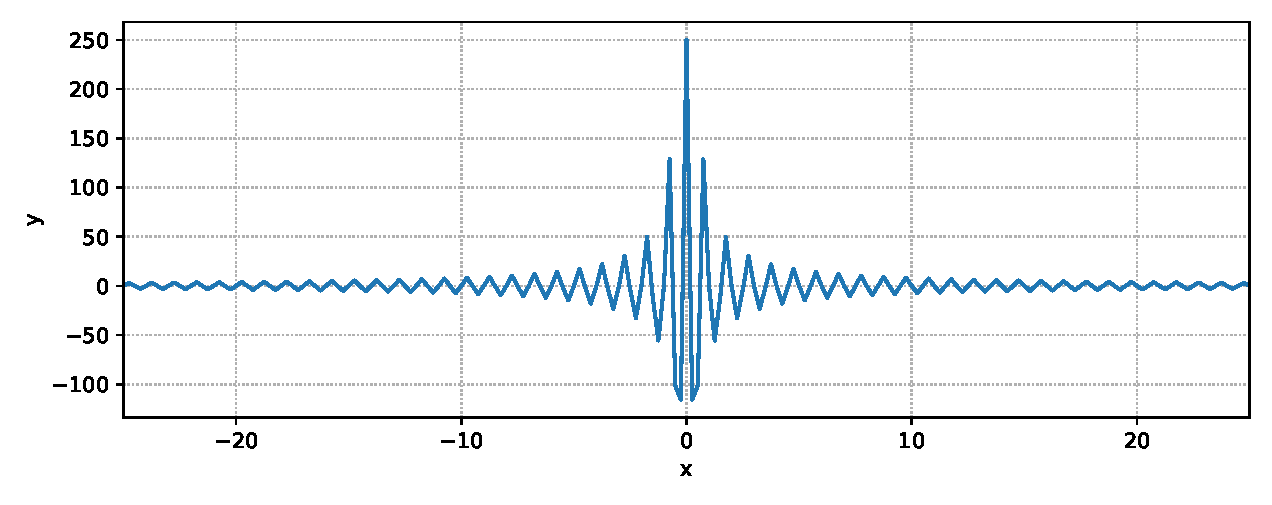
\includegraphics[width=1.0\textwidth]{./fig1.pdf}
  \caption{This a dummy figure to be replaced.}
  \label{fig:dummyfigure}
\end{figure*}

Figure \ref{fig:dummyfigure} shows how to include a figure.
Table \ref{tab:dummytable} shows how to include a table.

\bigskip

\lipsum[2-3]

\section{Results}
\subsection{Simulation results}

\lipsum[2]

\subsection{Other results}
\lipsum[2]

% example table
\begin{table}
  \centering
  \begin{tabular}{lrrr}
  \toprule
  $\alpha$   & $\beta$ & $\gamma$ & $\delta$ \\
  \midrule
  A          & 1       & a        & 3        \\
  B          & 2       & b        & 2        \\
  C          & 3       & c        & 1        \\
  \bottomrule
  \end{tabular}
  \caption{This is a dummy table to be replaced.}
  \label{tab:dummytable}
\end{table}



\section{Discussion}
\lipsum[2]


\section{Conclusion}
\lipsum[2]





%-------------------------------------------------------------------------------------------
\printbibliography
\color{red}Please specify DOIs if possible.
\end{document}
